
\documentclass{article}
\usepackage{amsmath, enumitem}
\usepackage{graphicx}

\usepackage{booktabs}
\usepackage{tabularx}
\usepackage[margin=1in]{geometry}


\begin{document}

\title{Econ 741 Homework 3}
\author{John Appert, Randall Chicolla, Andrea Franz}
\maketitle

\section{Question 1:  Polynomials (Stata)}
Let’s see how income varies with age. First construct your sample. We will want to
study individuals who are (inclusively) between 16 and 65 years of age, have positive earnings, and worked more than 1000 hours in a year. Pick a polynomial specification (of age) to run.

\begin{enumerate}[label=\alph*]
\item Present the results from your regression.  (5 points)

Answer:\\
%For some reason Table 1: Poly Regr Outputs at bottom of page. Can't figure out how to get it under part A

\begin{table}[tbp] \centering
\newcolumntype{C}{>{\centering\arraybackslash}X}

\caption{Poly Regression}
\begin{tabularx}{\textwidth}{lCCCC}

\toprule
{var}&{coef}&{stderr}&{N}&{r2} \tabularnewline
\midrule\addlinespace[1.5ex]
age&-15531.65&1854.559&1331847&.0781559 \tabularnewline
age2&1094.551&101.1481&1331847&.0781559 \tabularnewline
age3&-29.11097&2.645224&1331847&.0781559 \tabularnewline
age4&.3464887&.0332961&1331847&.0781559 \tabularnewline
age5&-.0015639&.000162&1331847&.0781559 \tabularnewline
\_cons&67744.05&13003.67&1331847&.0781559 \tabularnewline
\bottomrule \addlinespace[1.5ex]

\end{tabularx}
\end{table}


\item Explain why you picked the specification you did.  (6 points)

Looking at the twoway scatter (age incwage), it appeared visually that there might be a cubic. Also looking at the Adjusted R sqr increasing when adding polynomial terms and we check to see if adding polynomial terms adds anything to the regression when looking at the coefficients. Finally, ovtest was used to check if we were had omitted any polynomials.

Our specification:\\
reg incwage age age2 age3 age4 age5

%insert twoway scatter
\begin{figure}
\caption{\label {age incwage}}
\includegraphics[scale=1]{age_inwage_graph.pdf}
\end{figure}
%Still shows in the wrong spot

\item  Give the marginal effect and the average of the marginal effects. 
We also looked at a WALD test the null that the beta coefficientsw were equal to zero. (4 points)

We used the margins, dydx and atmeans commands.

Average Marginal Effects 
margins, dydx(age age2 age3 age4 age5)

\begin{table}[tbp] \centering
\newcolumntype{C}{>{\centering\arraybackslash}X}

\caption{Average Marginal Effects}
\begin{tabularx}{\textwidth}{lCCCC}

\toprule
{var}&{coef}&{stderr}&{N}&{r2} \tabularnewline
\midrule\addlinespace[1.5ex]
age&-15531.65&1854.559&1331847&.0781559 \tabularnewline
age2&1094.551&101.1481&1331847&.0781559 \tabularnewline
age3&-29.11097&2.645224&1331847&.0781559 \tabularnewline
age4&.3464887&.0332961&1331847&.0781559 \tabularnewline
age5&-.0015639&.000162&1331847&.0781559 \tabularnewline
\_cons&67744.05&13003.67&1331847&.0781559 \tabularnewline
\bottomrule \addlinespace[1.5ex]

\end{tabularx}
\end{table}




Marginal effects at the means
margins, dydx(age age2 age3 age4 age5) atmeans

\begin{table}[tbp] \centering
	\newcolumntype{C}{>{\centering\arraybackslash}X}
	
	\caption{Marginal Effects at the Mean}
	\begin{tabularx}{\textwidth}{lCCCC}
		
		\toprule
		{var}&{coef}&{stderr}&{N}&{r2} \tabularnewline
		\midrule\addlinespace[1.5ex]
		age&-15531.65&1854.559&1331847&.0781559 \tabularnewline
		age2&1094.551&101.1481&1331847&.0781559 \tabularnewline
		age3&-29.11097&2.645224&1331847&.0781559 \tabularnewline
		age4&.3464887&.0332961&1331847&.0781559 \tabularnewline
		age5&-.0015639&.000162&1331847&.0781559 \tabularnewline
		\_cons&67744.05&13003.67&1331847&.0781559 \tabularnewline
		\bottomrule \addlinespace[1.5ex]
		
	\end{tabularx}
\end{table}


\item  Discuss the significance of your polynomial overall as well as the individual terms.  (4 points)

reg incwage age age2 age3 age4 age5 Overall: \\

Adj R2 overall is .0782 which is not very explanatory, so we likely need more variables since a lot is left unexplained.
The F-test of our model. Prob > F =0.0000 tells us that H0 that the R^2=0 (that our model is no good explains
none of the variation in our dependent variable). Say we could say it is statistically significant at all confidence levels.

Individual terms: Looking at Wald test, low p-values indicate 
the null (that the beta coefficients are 0) should be rejected. That is that 
they are meaningful additions .

Looking at the t-statistics, (xbar - mu)/ (s\sqrt(n)) or signal to Noise, we have 
relatively large t-stat values so combined with the low pvalues tells us the H0 
(coefficient of variable equals zeros)



\end{enumerate}

\section{Question 2:  Indicator Variables and Interactions  (Stata)}
Let’s now see how earnings varies with marriage. Use the marst variable to create
three indicator variables for whether people are a) never married b) currently married c) formerly married.

\begin{enumerate}[label=\alph*]
\item  Put all three indicator variables into your model. Discuss the results. (6 points)

We used tab marst, nolab to determine categorical labels and then tried a similar method from class using 
gen and replace commands with an or statement to six categories into three new buckets. Something seemed off.
We regressed three and got multicolinearity as one expects putting all dummies in, but also had it in the regression 
with just two out of three dummies.\\

So we tried another method, tab marst, g(m) and then renamed the variables. Then generating the three indicator variables seemed to work,
when we put in only two. Putting in all three resulted in multicollinearity as we would expect.

\begin{table}[tbp] \centering
	\newcolumntype{C}{>{\centering\arraybackslash}X}
	
	\caption{Indicator Variable Regression}
	\begin{tabularx}{\textwidth}{lCCCC}
		
		\toprule
		{var}&{coef}&{stderr}&{N}&{r2} \tabularnewline
		\midrule\addlinespace[1.5ex]
		age&-15531.65&1854.559&1331847&.0781559 \tabularnewline
		age2&1094.551&101.1481&1331847&.0781559 \tabularnewline
		age3&-29.11097&2.645224&1331847&.0781559 \tabularnewline
		age4&.3464887&.0332961&1331847&.0781559 \tabularnewline
		age5&-.0015639&.000162&1331847&.0781559 \tabularnewline
		\_cons&67744.05&13003.67&1331847&.0781559 \tabularnewline
		\bottomrule \addlinespace[1.5ex]
		
	\end{tabularx}
\end{table}

\item Run a model that will test whether or not married people see their wages go up
more quickly with age than people who were never married. Discuss the results.
(8 points)

gen ageNM= age*NM
reg incwage age age2 age3 age4 age5 NM CM 

Running this gave us results.

\begin{table}[tbp] \centering
	\newcolumntype{C}{>{\centering\arraybackslash}X}
	
	\caption{Interaction Regression}
	\begin{tabularx}{\textwidth}{lCCCC}
		
		\toprule
		{var}&{coef}&{stderr}&{N}&{r2} \tabularnewline
		\midrule\addlinespace[1.5ex]
		age&-6089.086&1847.886&1331847&.0910964 \tabularnewline
		age2&607.7899&100.9341&1331847&.0910964 \tabularnewline
		age3&-17.30284&2.641194&1331847&.0910964 \tabularnewline
		age4&.2097509&.0332475&1331847&.0910964 \tabularnewline
		age5&-.0009531&.0001617&1331847&.0910964 \tabularnewline
		NM&18866.36&514.2944&1331847&.0910964 \tabularnewline
		CM&16968.16&162.5083&1331847&.0910964 \tabularnewline
		ageNM&-417.7659&12.14724&1331847&.0910964 \tabularnewline
		\_cons&-11567.8&12931.09&1331847&.0910964 \tabularnewline
		\bottomrule \addlinespace[1.5ex]
		
	\end{tabularx}
\end{table}

\end{enumerate}

\section{Question 3:  Functional Form (Stata)}
Construct a variable that is years of education. Report and interpret (in one sentence each) the following coefficients with a model of earnings on education:

\begin{enumerate}[label=\alph*]

\item Linear-Linear (4 points)

reg incwage i.educ

\begin{table}[tbp] \centering
	\newcolumntype{C}{>{\centering\arraybackslash}X}
	
	\caption{Linear-Linear Regression}
	\begin{tabularx}{\textwidth}{lCCCC}
		
		\toprule
		{var}&{coef}&{stderr}&{N}&{r2} \tabularnewline
		\midrule\addlinespace[1.5ex]
		0b.educ&0&0&1331847&.1458944 \tabularnewline
		1.educ&-2399.32&1026.261&1331847&.1458944 \tabularnewline
		2.educ&-2698.808&667.6634&1331847&.1458944 \tabularnewline
		3.educ&-4883.14&737.1592&1331847&.1458944 \tabularnewline
		4.educ&-7426.246&687.9224&1331847&.1458944 \tabularnewline
		5.educ&-9334.577&645.1861&1331847&.1458944 \tabularnewline
		6.educ&5257.943&539.4581&1331847&.1458944 \tabularnewline
		7.educ&8886.766&546.7324&1331847&.1458944 \tabularnewline
		8.educ&15787.23&556.1182&1331847&.1458944 \tabularnewline
		10.educ&39498.69&542.6752&1331847&.1458944 \tabularnewline
		11.educ&70093.13&549.3376&1331847&.1458944 \tabularnewline
		\_cons&29815.12&532.5793&1331847&.1458944 \tabularnewline
		\bottomrule \addlinespace[1.5ex]
		
	\end{tabularx}
\end{table}



\item Log-Linear (4 points)

gen LNincwage=ln(incwage)
reg LNincwage i.educ


\begin{table}[tbp] \centering
	\newcolumntype{C}{>{\centering\arraybackslash}X}
	
	\caption{Log-Linear Regression}
	\begin{tabularx}{\textwidth}{lCCCC}
		
		\toprule
		{var}&{coef}&{stderr}&{N}&{r2} \tabularnewline
		\midrule\addlinespace[1.5ex]
		0b.educ&0&0&1331847&.1458944 \tabularnewline
		1.educ&-2399.32&1026.261&1331847&.1458944 \tabularnewline
		2.educ&-2698.808&667.6634&1331847&.1458944 \tabularnewline
		3.educ&-4883.14&737.1592&1331847&.1458944 \tabularnewline
		4.educ&-7426.246&687.9224&1331847&.1458944 \tabularnewline
		5.educ&-9334.577&645.1861&1331847&.1458944 \tabularnewline
		6.educ&5257.943&539.4581&1331847&.1458944 \tabularnewline
		7.educ&8886.766&546.7324&1331847&.1458944 \tabularnewline
		8.educ&15787.23&556.1182&1331847&.1458944 \tabularnewline
		10.educ&39498.69&542.6752&1331847&.1458944 \tabularnewline
		11.educ&70093.13&549.3376&1331847&.1458944 \tabularnewline
		\_cons&29815.12&532.5793&1331847&.1458944 \tabularnewline
		\bottomrule \addlinespace[1.5ex]
		
	\end{tabularx}
\end{table}




\item Linear-Log (4 points)

gen LNeduc=ln(educ)
reg incwage LNeduc


\begin{table}[tbp] \centering
	\newcolumntype{C}{>{\centering\arraybackslash}X}
	
	\caption{Linear-Log Regression}
	\begin{tabularx}{\textwidth}{lCCCC}
		
		\toprule
		{var}&{coef}&{stderr}&{N}&{r2} \tabularnewline
		\midrule\addlinespace[1.5ex]
		0b.educ&0&0&1331847&.1458944 \tabularnewline
		1.educ&-2399.32&1026.261&1331847&.1458944 \tabularnewline
		2.educ&-2698.808&667.6634&1331847&.1458944 \tabularnewline
		3.educ&-4883.14&737.1592&1331847&.1458944 \tabularnewline
		4.educ&-7426.246&687.9224&1331847&.1458944 \tabularnewline
		5.educ&-9334.577&645.1861&1331847&.1458944 \tabularnewline
		6.educ&5257.943&539.4581&1331847&.1458944 \tabularnewline
		7.educ&8886.766&546.7324&1331847&.1458944 \tabularnewline
		8.educ&15787.23&556.1182&1331847&.1458944 \tabularnewline
		10.educ&39498.69&542.6752&1331847&.1458944 \tabularnewline
		11.educ&70093.13&549.3376&1331847&.1458944 \tabularnewline
		\_cons&29815.12&532.5793&1331847&.1458944 \tabularnewline
		\bottomrule \addlinespace[1.5ex]
		
	\end{tabularx}
\end{table}



\item Log-Log (4 points)


\begin{table}[tbp] \centering
	\newcolumntype{C}{>{\centering\arraybackslash}X}
	
	\caption{Log-Log Regression}
	\begin{tabularx}{\textwidth}{lCCCC}
		
		\toprule
		{var}&{coef}&{stderr}&{N}&{r2} \tabularnewline
		\midrule\addlinespace[1.5ex]
		0b.educ&0&0&1331847&.1458944 \tabularnewline
		1.educ&-2399.32&1026.261&1331847&.1458944 \tabularnewline
		2.educ&-2698.808&667.6634&1331847&.1458944 \tabularnewline
		3.educ&-4883.14&737.1592&1331847&.1458944 \tabularnewline
		4.educ&-7426.246&687.9224&1331847&.1458944 \tabularnewline
		5.educ&-9334.577&645.1861&1331847&.1458944 \tabularnewline
		6.educ&5257.943&539.4581&1331847&.1458944 \tabularnewline
		7.educ&8886.766&546.7324&1331847&.1458944 \tabularnewline
		8.educ&15787.23&556.1182&1331847&.1458944 \tabularnewline
		10.educ&39498.69&542.6752&1331847&.1458944 \tabularnewline
		11.educ&70093.13&549.3376&1331847&.1458944 \tabularnewline
		\_cons&29815.12&532.5793&1331847&.1458944 \tabularnewline
		\bottomrule \addlinespace[1.5ex]
		
	\end{tabularx}
\end{table}



\end{enumerate}

\section{Question 4:  Heteroskedasticity (Stata and R)}

\begin{enumerate}[label=\alph*]

\item Is there evidence of heteroskedasticity based on age? Show me in a picture.
Discuss. (12 points)\\




Yes.  If there were no heteroskedasticity in the data the residuals plotted against the independent variable would be random.  In the figure below we see that there is an upward curve in the data.  It is certainly not random.  Therefore the data shows clear heteroskedasticity.


\begin{figure}[ht!]
\centering
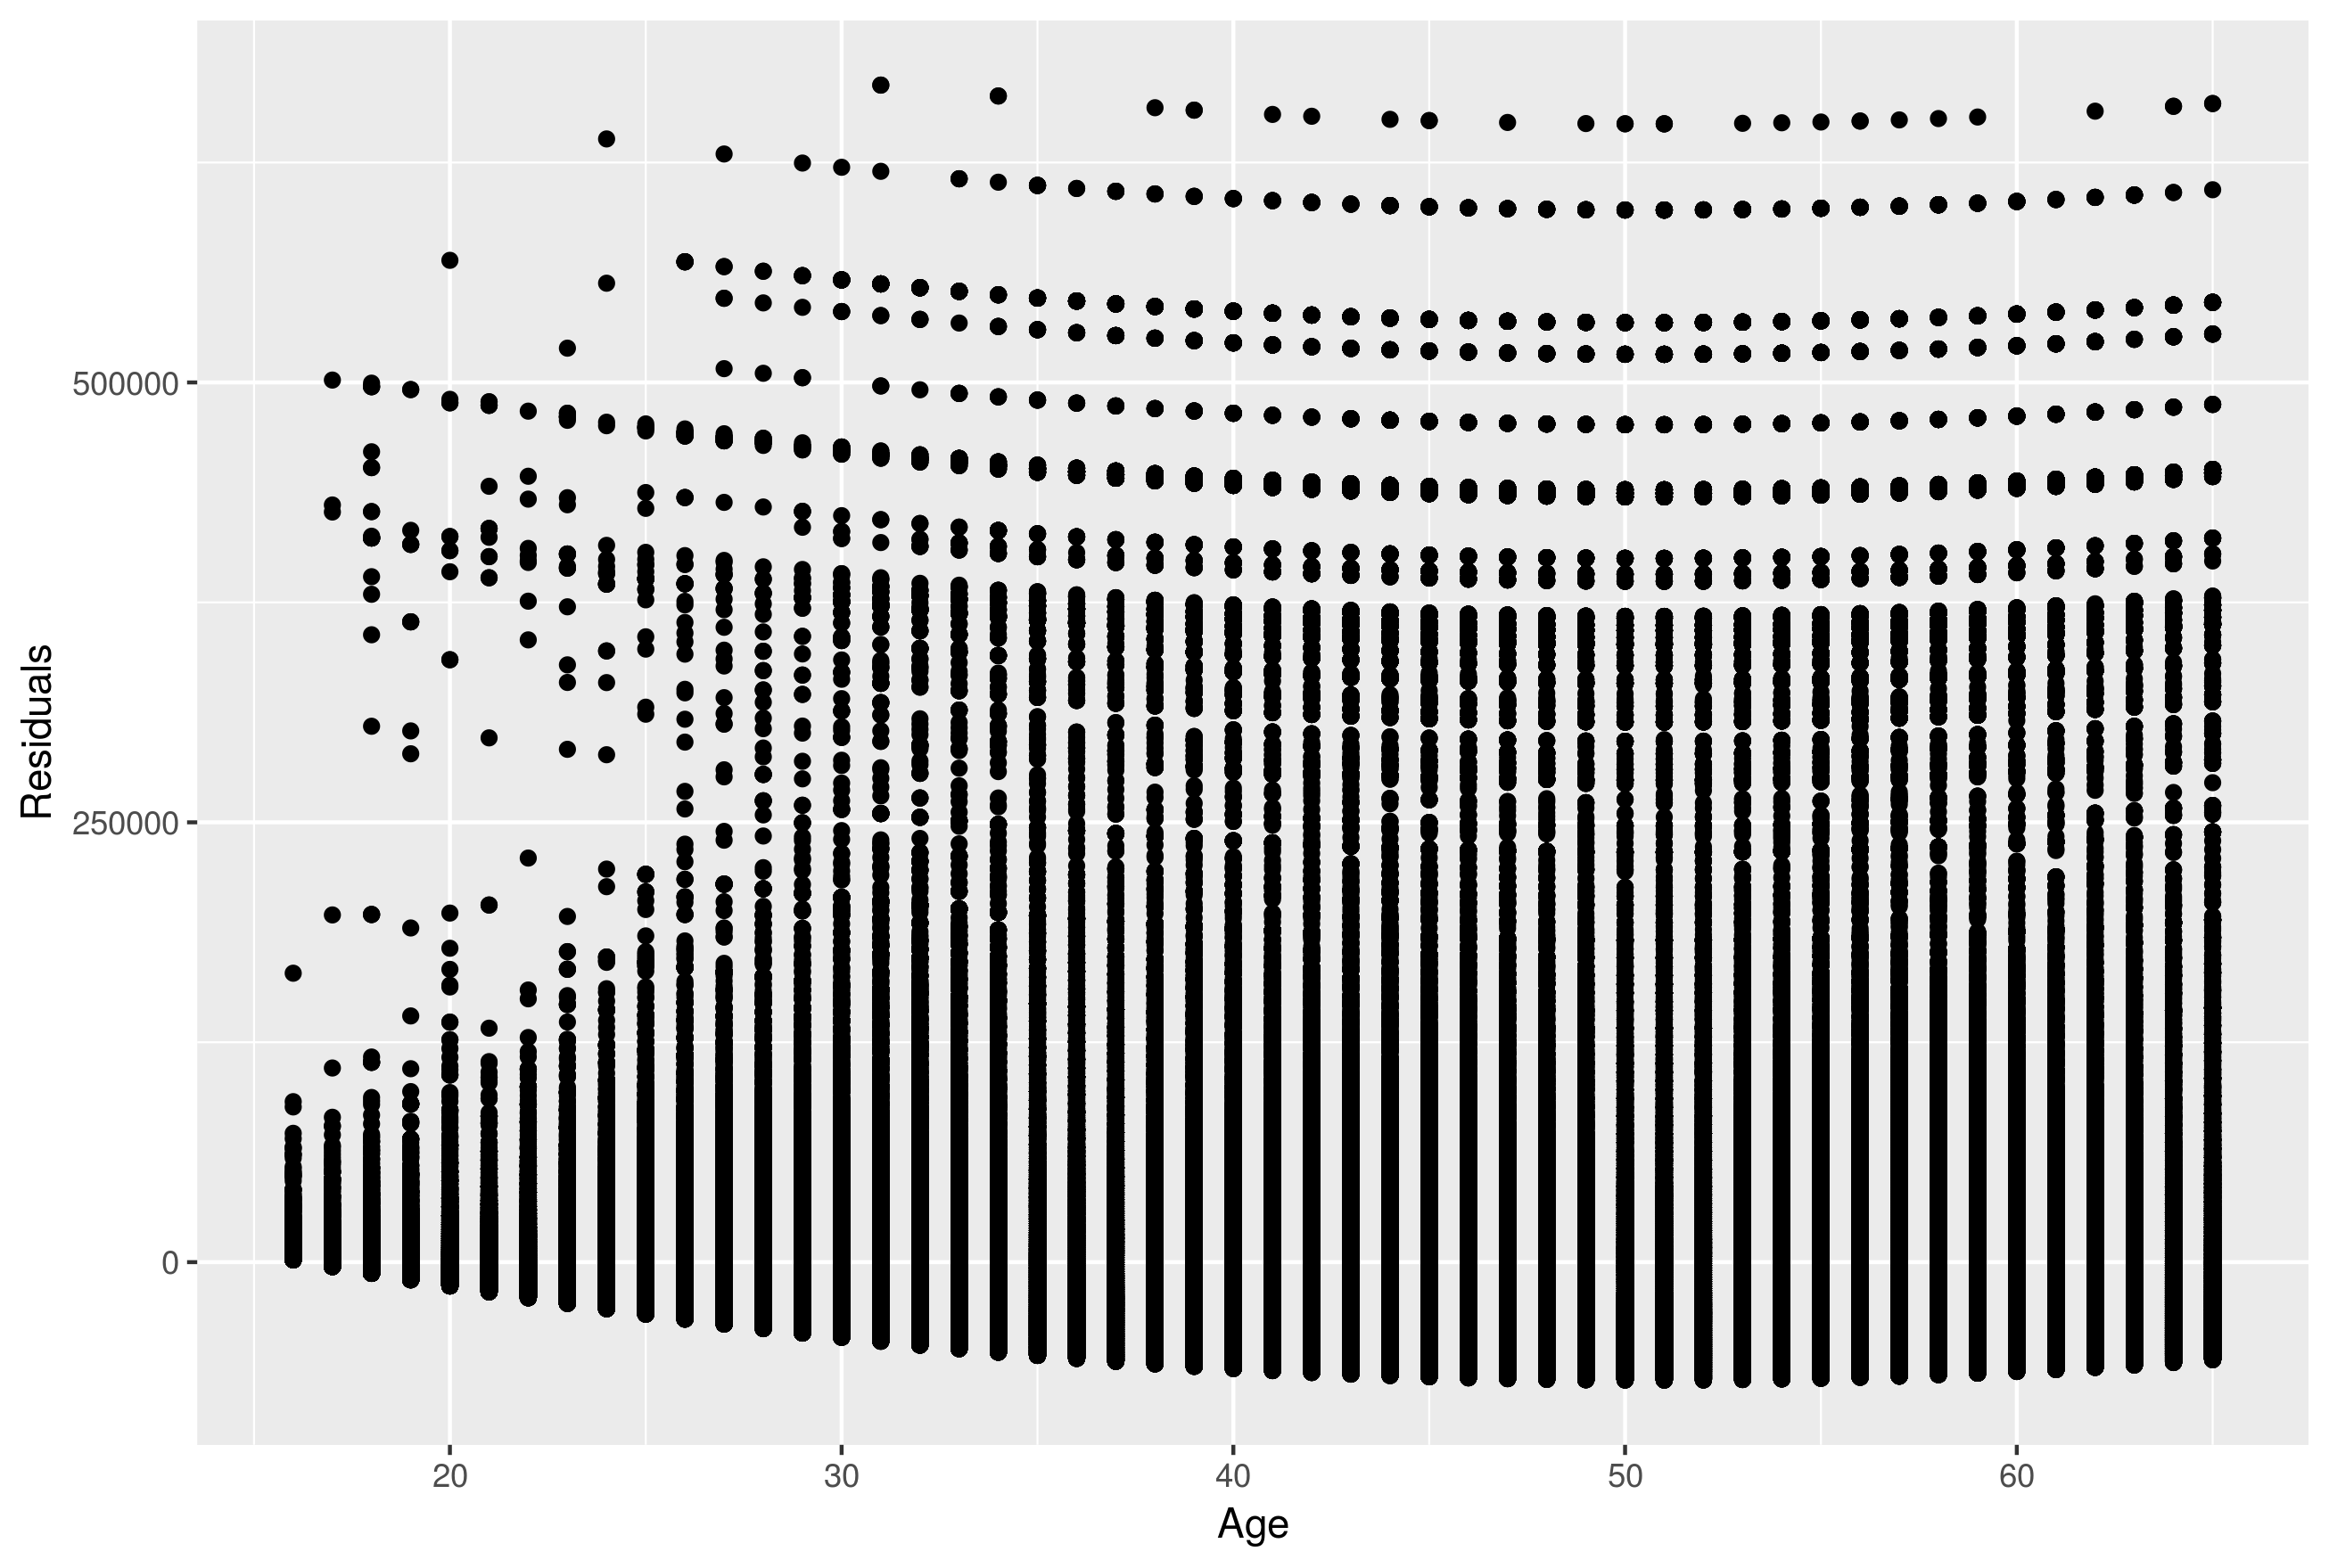
\includegraphics[width=90mm]{residuals.png}
\caption{Residuals vs Age \label{overflow}}
\end{figure}

This compares with our Stata plot of squared errors to the linear prediction.\\

\begin{figure}[ht!]
	\centering
	\includegraphics[width=90mm]{e2_yhat.pdf}
	\caption{Residuals vs Age \label{overflow}}
\end{figure}



\item Obtain robust standard errors in R and Stata. (18 points)

The values of the robust standard errors found in R were as follows:\\
With no adjustment for degrees of freedom:

Age:  23.6251\\
Age2:  0.3024647\\
Cons:  399.5719148\\

We adjusted these values for the degrees of freedom using:

$ N/(N-k)$

Age:  23.625128\\
Age2:  0.302465 \\
Cons:  399.572365\\

Using Stata we found the following values for robust standard errors:

Age:  23.62513\\
Age2:  0.302465 \\
Cons:  399.5724\\

\begin{table}[tbp] \centering
	\newcolumntype{C}{>{\centering\arraybackslash}X}
	
	\caption{Robust Regression}
	\begin{tabularx}{\textwidth}{lCCCC}
		
		\toprule
		{var}&{coef}&{stderr}&{N}&{r2} \tabularnewline
		\midrule\addlinespace[1.5ex]
		age&5742.326&23.62513&1331847&.0777715 \tabularnewline
		age2&-56.60501&.302465&1331847&.0777715 \tabularnewline
		\_cons&-78621.34&399.5724&1331847&.0777715 \tabularnewline
		\bottomrule \addlinespace[1.5ex]
		
	\end{tabularx}
\end{table}

\end{enumerate}
\end{document}
